\section{Poisson equation with PETSc}
  \label{section:applications:petsc}

\chapterDescription
  {
    60 minutes.
  }
  {
    Chapter \ref{chapter:quickstart} and a working PETSc installation.
  }

I wrote Peano with matrix-free methods for computational fluid dynamics in mind. 
It turns out that it is not too complicated to use it for other application
areas or to established linear algebra packages.
We assume that you have PETSc plus BLAS, Lapack and MPI (if required) ready
installed on your system.
I have tested all the present concepts with PETSc 3.7.2 but everything discussed
here is pretty basic, so it should work with older versions as well.
Please note that this is a feasibility study and we do not optimise at all.


\subsection{Preparation of Peano}

If we use explicit assembly, we need an enumeration of our grid. 
So we do start with a grid
\begin{code}
> java -jar <mypath>/pdt.jar --create-project petsc chapter-4.3
\end{code}

\noindent
and add each vertex an index. 
We do restrict to a discretisation with one degree of freedom per vertex for the
time being:

\begin{code}
Packed-Type: short int;

class petsc::records::Vertex {  
  parallelise persistent int index;
};
\end{code}

\noindent
For the present exercise, we will have four different things to do:
create the grid, create and assemble the matrix, solve the problem and plot the
result.
The solve is a pure PETSc operation.
For each of the remaining three phases, we need a mapping/adapter in Peano and
we also want access to \texttt{index}.
For the latter, we could write setters and getters and stick to an
object-oriented paradigm.
But this way, it is easier (though not as beautiful):

\begin{code}
component: MyFancyPETScProject

namespace: ::petsc

vertex:
  dastgen-file: Vertex.def
  read scalar(int): Index   // mind the uppercase
  write scalar(int): Index
  
cell:
  dastgen-file: Cell.def

state:
  dastgen-file: State.def

event-mapping:
  name: CreateGrid

event-mapping:
  name: Assemble

adapter:
  name: CreateGrid
  merge-with-user-defined-mapping: CreateGrid

adapter:
  name: Assemble
  merge-with-user-defined-mapping: Assemble
 
adapter:
  name: Plot
  merge-with-predefined-mapping: VTKPlotVertexValue(result,getU,u)
\end{code}

We generate all glue code
\begin{code}
> java -jar <mypath>/pdt.jar --generate-gluecode \
  petsc/project.peano-specification petsc <mypath>/pdt/usrtemplates
> make -f petsc/makefile
\end{code}

\noindent
We recognise that this code does not compile yet as we have not yet realised \texttt{double Vertex::getU() const}.
For the time being, we make the routine return 0.
Finally, we change into the mapping the creational events yield a regular grid:

\begin{code}
void petsc::mappings::CreateGrid::createInnerVertex(...) {
  logTraceInWith6Arguments( "createInnerVertex(...)", ... );

  if (coarseGridVerticesEnumerator.getLevel()<3) {
	fineGridVertex.refine();
  }

  logTraceOutWith1Argument( "createInnerVertex(...)", fineGridVertex );
}


void petsc::mappings::CreateGrid::createBoundaryVertex(...) {
  logTraceInWith6Arguments( "createBoundaryVertex(...)", ... );

  if (coarseGridVerticesEnumerator.getLevel()<3) {
	fineGridVertex.refine();
  }

  logTraceOutWith1Argument( "createBoundaryVertex(...)", fineGridVertex );
}
\end{code}

\noindent
Compile it, run it, visualise the output.


\subsection{Connecting to PETSc}

As PETSc's philosophy is pretty straightforward and minimalistic (they do, e.g.,
not hijack the main), the initialisation and integration are straightforward.
Please note that we stick to serial jobs in the first part of this section.
Nevertheless, we use the MPI compiler wrapper to translate the code as I faced
issues when I tried to use PETSc without MPI\footnote{Please consult
\url{http://www.mcs.anl.gov/petsc/petsc-current/docs/installation.html#i-dont-want-to-use-mpi}
for the usage with OpenMPI as the \texttt{LD\_LIBRARY\_PATH} has to be set
properly.}.


\begin{enumerate}
  \item Before we start to code with PETSc, we have to make the makefile know
  where PETSc is installed. If you use your own build environment, adopt all
  pathes accordingly. If you use the pre-generated makefile, open it and add
  your PETSc include directory to the search path. Also switch to
  \texttt{mpiCC}.
  \begin{code}
    PROJECT_CFLAGS = -DDebug -DAsserts -DParallel \
      -DMPICH_IGNORE_CXX_SEEK -I/opt/petsc/include 
    PROJECT_LFLAGS = -L/opt/petsc/lib -lpetsc 
    PROJECT_LFLAGS = -L/opt/petsc/lib -lpetsc

    [...]

    CC=/opt/openmpi/bin/mpiCC
  \end{code}
  Please adopt all pathes accordingly. Depending on your MPI version, you also
  might run into issues with the compiler's error management. I recommend to
  remove \texttt{-Werror -pedantic-errors} from your makefile in this case.
  \item As the present PETSc solutions use MPI (through they run serially), we
  have to make a few modifications in the runner. These modifications are
  detailed in Chapter \ref{section:parallelisation:mpi}, so we simply show
  what has to be changed in \texttt{runners/Runner.cpp}. This solution should
  work out-of-the-box.
  For a description of its semantics, please see the aforementioned chapter.
  \begin{code}
#include "tarch/parallel/FCFSNodePoolStrategy.h"
#include "peano/parallel/loadbalancing/OracleForOnePhaseWithGreedyPartitioning.h"

[...]

int petsc::runners::Runner::run() {

  [...]

  petsc::repositories::Repository* repository = 
    petsc::repositories::RepositoryFactory::getInstance().createWithSTDStackImplementation(
      geometry,
      tarch::la::Vector<DIMENSIONS,double>(1.0),   // domainSize,
      tarch::la::Vector<DIMENSIONS,double>(0.0)    // computationalDomainOffset
    );
  

  // This is new because of PETSc:
  if (tarch::parallel::Node::getInstance().isGlobalMaster()) {
    tarch::parallel::NodePool::getInstance().setStrategy(
      new tarch::parallel::FCFSNodePoolStrategy()
    );
  }
  tarch::parallel::NodePool::getInstance().restart();
  tarch::parallel::NodePool::getInstance().waitForAllNodesToBecomeIdle();
  peano::parallel::loadbalancing::Oracle::getInstance().setOracle(
    new peano::parallel::loadbalancing::OracleForOnePhaseWithGreedyPartitioning(false)
  );

  [...]
}
  \end{code}
  \item Finally, we have to initialise and shut down PETSc properly in
  \texttt{main.cpp}:
  \begin{code}
#include "petscsys.h"

[...]

int main(int argc, char** argv) {
  [...]
  PetscInitialize(&argc,&argv,(char*)0,(char*)0);

  int programExitCode = 0;

  if (programExitCode==0) {
    [...]
    petsc::runners::Runner runner;
    programExitCode = runner.run();
  }

  PetscFinalize();
  [...]
}  
  \end{code}
  According to PETSc's documentation, we could use PETSc's initialisation to set
  up MPI instead of the Peano initialisation. However, Peano's initialisation
  does not check whether MPI has been set up before where PETSc does. So it
  makes sense to initialise Peano first.
\end{enumerate}




\subsection{Letting PETSc do the work}

Once we have created the grid (and perhaps visualised it), we can start to set
up the PETSc data structures corresponding to the grid, we can call its solver,
and we can finally free everything afterwards.
We stick to the regular case for the time being.

Every fine grid vertex in the grid has a right-hand side and a solution entry. 
Different to previous sections, we do not store this data in the vertex.
Instead, we will make PETSc hold two vectors $rhs$ and $x$ and
make each vertex hold the index, i.e.~each vertex knows which entry in the two
vertices is associated with the vertex.
So this means that the runner has to create these vectors and destroy them
afterwards as well:

\begin{code}
  thisIsATest++;
\end{code}

\begin{code}
#include "petscvec.h"
#include "petscmat.h"

[...]

int petsc::runners::Runner::runAsMaster(petsc::repositories::Repository& repository) {
  peano::utils::UserInterface::writeHeader();

  // Build up the grid. Afterwards, we know how many vertices exist.
  repository.switchToCreateGrid(); repository.iterate();


  // These are the global vectors that we use to make the adapter communicate with PETSc:
  Vec  x;
  Vec  rhs;
  Mat  A;

  // Create the global vector required for our work with PETSc.
  PetscErrorCode errorX   = 
    VecCreate(tarch::parallel::Node::getInstance().getCommunicator(), &x);
  PetscErrorCode errorRhs = 
    VecCreate(tarch::parallel::Node::getInstance().getCommunicator(), &rhs);
  PetscErrorCode errorA   = 
    MatCreate(tarch::parallel::Node::getInstance().getCommunicator(), &A);

  if (errorX!=0) {
    PetscError( tarch::parallel::Node::getInstance().getCommunicator(),
      __LINE__,  __FUNCT__,  __FILE__, errorX,  PETSC_ERROR_INITIAL,
      "creating global solution vector failed" );
  }
  if (errorRhs!=0) {
    PetscError( tarch::parallel::Node::getInstance().getCommunicator(),
      __LINE__,  __FUNCT__,  __FILE__, errorRhs,  PETSC_ERROR_INITIAL,
      "creating global rhs vector failed" );
  }
  if (errorA!=0) {
    PetscError( tarch::parallel::Node::getInstance().getCommunicator(),
      __LINE__,  __FUNCT__,  __FILE__, errorA,  PETSC_ERROR_INITIAL,
      "creating system matrix failed" );
  }


  // Local size (first parameter) and global size are the same for the time
  // being. Peano uses doubles to count vertices, as the number of vertices
  // sometimes exceed int. So we have to use an ugly cast here.
  const PetscInt numberOfUnknowns = static_cast<int>(
    repository.getState().getNumberOfInnerLeafVertices());

  assertion1( numberOfUnknowns>0, numberOfUnknowns );

  VecSetSizes(x,  PETSC_DECIDE,numberOfUnknowns);
  VecSetSizes(rhs,PETSC_DECIDE,numberOfUnknowns);
  VecSetType(x,VECMPI);
  VecSetType(rhs,VECSEQ);
  MatSetSizes(A,PETSC_DECIDE,PETSC_DECIDE,numberOfUnknowns,numberOfUnknowns);
  MatSetType(A,MATSEQAIJ);
  MatSetUp(A);
  
  repository.switchToAssemble(); repository.iterate();

  // @todo Do the real solve here

  repository.switchToPlot(); repository.iterate();


  // Clean up PETSc data structures
  VecDestroy(&x);
  VecDestroy(&rhs);
  MatDestroy(&A);

  repository.logIterationStatistics( true );
  repository.terminate();

  return 0;
}
\end{code}

\noindent
That's basically the structure of our whole solver.
What is missing is to set up the system matrix and to befill the $rhs$ vector.
For this, we have to ensure that the assembly process (and also the plot later
on) know the respective data structures.
For convenience, I thus recommend to move the three important data variables
into \texttt{Vertex.h}:

\begin{code}
#include "petscvec.h"
#include "petscmat.h"


namespace petsc { 
  class Vertex;
      
  // Forward declaration
  class VertexOperations;

  // These are the global vectors that we use to make the adapter communicate
  // with PETSc:
  extern Vec  x;
  extern Vec  rhs;
  extern Mat  A;
}
\end{code}

\noindent
Please note that we move these variables, i.e.~their declaration has to be
removed from \texttt{runAsMaster}. Furthermore, we have to add their definition
to \texttt{Vertex.cpp}:

\begin{code}
Vec  petsc::x;
Vec  petsc::rhs;
Mat  petsc::A;
\end{code}

We finally have to solve the actual equation system in the runner. For this, we
plug into the \texttt{@todo} from the snippet above and furthermore include
\texttt{\#include "petscksp.h"}. We use a simple Krylov CG solver here with a
diagonal value preconditioner.

\begin{code}
KSP krylovSolver;
PC  preconditioner;

KSPCreate(tarch::parallel::Node::getInstance().getCommunicator(),&krylovSolver);
KSPSetOperators(krylovSolver,A,A); // use matrix from Vector.h

// connect/get preconditioner
KSPGetPC(krylovSolver,&preconditioner);

// set Jacobi as preconditioner
PCSetType(preconditioner,PCBJACOBI);

KSPSolve(krylovSolver,rhs,x);
KSPDestroy(&krylovSolver);
\end{code}

\noindent
This is not a particular sophisticated code, but it does the job. 
No need to rewrite parts of the excellent PETSc documentation.

\subsection{Connecting the vertices to PETSc}

We next have to couple the vertices from our grid to the PETSc unknowns. 
For this, we add a field     

\begin{code}
int  _unknownCounter;
\end{code}

\noindent
to the class \texttt{Assemble} and make each fine grid vertex hold a unique
index which is basically the corresponding entry in the $x$ and $rhs$ vector.
If we do so, we can also set $rhs$ already.

\begin{code}
#include "petsc/VertexOperations.h"

void petsc::mappings::Assemble::beginIteration(
  petsc::State&  solverState
) {
  logTraceInWith1Argument( "beginIteration(State)", solverState );

  _unknownCounter = 0;

  logTraceOutWith1Argument( "beginIteration(State)", solverState);
}

void petsc::mappings::Assemble::touchVertexFirstTime(
  ...
) {
  logTraceInWith6Arguments( "touchVertexFirstTime(...)", ... );

  if (
    fineGridVertex.getRefinementControl()==Vertex::Records::Unrefined
    &&
    fineGridVertex.isInside() // it is not a boundary point
  ) {
    VertexOperations::writeIndex(fineGridVertex,_unknownCounter);
    _unknownCounter++;
    
    fineGridVertex.setRhs( 1.0 ); // See routines below
  }

  logTraceOutWith1Argument( "touchVertexFirstTime(...)", fineGridVertex );
}
\end{code}

\noindent
There are many technical ways to couple the vertex to PETSc.
We do it via the vertices:

\begin{code}
double petsc::Vertex::getU() const {
  double result = 0.0;
  if (isInside()) {
    PetscInt     indices[] = {_vertexData.getIndex()};
    PetscScalar  values[]  = {0.0};

    VecGetValues(x,1,indices,values);

    result = values[0];
  }
  return result;
}


void petsc::Vertex::setRhs(double value) {
  PetscInt     indices[] = {_vertexData.getIndex()};
  PetscScalar  values[]  = {value};
  VecSetValues(rhs,1,indices,values, INSERT_VALUES);
}
\end{code}



\subsection{Assembling and retrieving data from PETSc}

We finally assemble our systems. The key activity is on the one hand to tell
PETSc that we have finished the assembly

\begin{code}
void petsc::mappings::Assemble::endIteration(
  petsc::State&  solverState
) {
  logTraceInWith1Argument( "endIteration(State)", solverState );

  logInfo( "beginIteration(State)", "finalise assembly" );

  VecAssemblyBegin( x );
  VecAssemblyBegin( rhs );
  VecAssemblyEnd( x );
  VecAssemblyEnd( rhs );

  MatAssemblyBegin(A, MAT_FINAL_ASSEMBLY);
  MatAssemblyEnd(A, MAT_FINAL_ASSEMBLY);

  logInfo( "beginIteration(State)", "assembly finished" );

  logTraceOutWith1Argument( "endIteration(State)", solverState);
}
\end{code}

\noindent
and on the other hand to fill entries into the matrix:
\begin{code}
#include "tarch/la/Matrix.h"


void petsc::mappings::Assemble::enterCell(
  ...
) {
 logTraceInWith4Arguments( "enterCell(...)", ... );

 if ( not fineGridCell.isRefined() ) {
  tarch::la::Matrix<4,4,double> localA;
  localA = 0.5,  -0.25, -0.25, 0,
           -0.25, 0.5,  0,    -0.25,
           -0.25, 0,    0.5,  -0.25,
           0,    -0.25, -0.25, 0.5;

  for(int ii=0; ii<4; ii++)
  for(int jj=0; jj<4; jj++) {
   if (
    fineGridVertices[fineGridVerticesEnumerator(ii)].isInside()
    &&
    fineGridVertices[fineGridVerticesEnumerator(jj)].isInside()
   ) {
    PetscInt row = VertexOperations::readIndex( fineGridVertices[fineGridVerticesEnumerator(ii)] );
    PetscInt col = VertexOperations::readIndex( fineGridVertices[fineGridVerticesEnumerator(jj)] );
    MatSetValue(A,row,col,localA(ii,jj),ADD_VALUES);
   }
  }
 }

 logTraceOutWith1Argument( "enterCell(...)", fineGridCell );
}
\end{code}

\noindent
Needless to say, this is a 2d example. 3d requires more indices. You might want
to have a look into the Peano utilities for dimension-generic routines. And it
is also obvious that this is not a very elegant and fast solution as we write
into the matrix entry by entry rather than in batches.

Once the matrix is assembled, it makes sense to add statements alike
\begin{code}
  KSPCreate(tarch::parallel::Node::getInstance().getCommunicator(),&krylovSolver);
  KSPSetOperators(krylovSolver,A,A); // use matrix from Vector.h
\end{code}

\noindent
into the runner to see the matrix pattern, e.g.



\subsection{Some remarks on discontinuous Galerkin}


\begin{figure}
  \begin{center}
    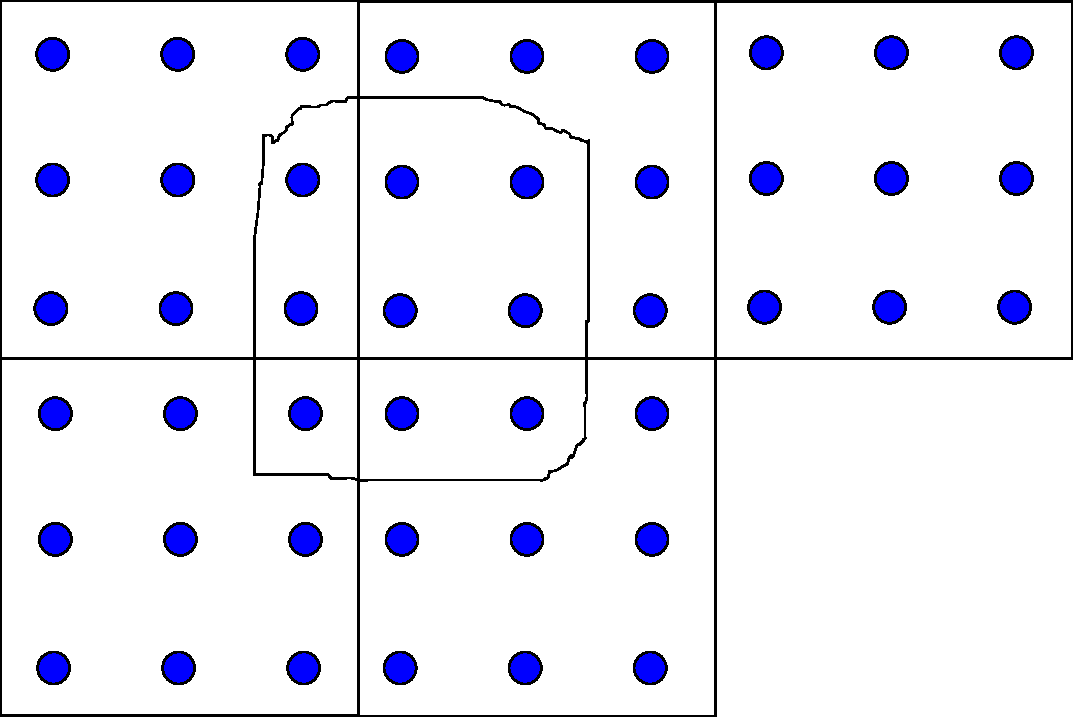
\includegraphics[width=0.6\textwidth]{43_dg/dg-data-layout.pdf}
  \end{center}
  \caption{One possible data layout for DG with PETSc. All indices are stored
  within vertices.}
  \label{figure:43_petsc:data-layout}
\end{figure}

There are various ways to implement discontinuous Galerkin in Peano. 
We sketch a vertex-based variant  at
hands of bi-quadratic shape functions.
For such an approach, we have to store nine unknown per cell.
However, we propose not to store indices within a cell but within vertices.
This is advantageous as we have, without additional effort, only vertices within
a cell at hand. 
We do not know neighbour cells.

So we propose to hold nine integer indices within each individual vertex.
Basically, every unknown is stored within its closest neighbouring vertex
(Figure \ref{figure:43_petsc:data-layout}). 
For those where multiple options do exist, we store it to the left bottom.
The corresponding vertex data structure reads as follows:
\begin{code}
Packed-Type: short int;

class petsc::records::Vertex {  
  parallelise persistent int index[9];
};
\end{code}



\subsection{Work in progress \ldots}

I am planning to start some programming with PETSc plus Peano plus MPI soon and
I also plan to dive into PETSc's matrix-free routines. If anybody reads this
comment and has suggestions, feel free to contact me.

\ldots to be continued



\subsection*{Further reading}

\begin{itemize}
  \item Weinzierl, Marion and Weinzierl, Tobias: {\em Quasi-matrix-free hybrid
  multigrid on dynamically adaptive Cartesian grids}, arXiv:1607.00648
\end{itemize}


% 
% 
% 
% \subsection{Serial assembly with a parallel PETSc}
% 
% 
% \subsection{Using PETSc and MPI}
% others. So it is a perfect fit to Peano.

